\section{Estimation of Physical Parameters from Radial Velocity Curves}

As an application so far, let us estimate the physical parameters 
$(V_\mathrm{sys}, K_\star, e, \omega, P, T_0)$ when radial velocity curve data 
${t_i, (v_r)_i} \ (i=1,2,\cdots,N)$ are given.  
First, the mean anomaly $M_i$ at the time $t_i$ is

\begin{align}
    M_i = (t_i - T_0) \dfrac{2 \pi}{P}
\end{align}

We can obtain $E_i$ from $M_i$ using the Newton-Raphson method.  
The corresponding true anomaly is related to $E$ by

\begin{align}
    \cos{f_i} &= \dfrac{\cos{E_i}-e}{1 - e \cos{E_i}} \\
    \sin{f_i} &= \dfrac{\sin{E_i} \sqrt{1-e^2}}{1 - e \cos{E_i}} 
\end{align}

From Eq.~(\ref{eq:vrsatarefinal}), we have

\begin{align}
&(v_r)_{i, \mathrm{model}} = \nonumber \\
&V_\mathrm{sys} + K_\star \left[ \cos{f_i} \cos{\omega} - \sin{f_i} \sin{\omega} + e \cos{\omega} \right] 
\end{align}

The probabilistic model assumes that the observational noise is independent Gaussian:

\begin{align}
    p(\dv|\thetav) &= \Ng(\muv, \sigma^2 I) \\
    \mu_i &= (v_r)_{i, \mathrm{model}} 
\end{align}

In this case, the parameters to be estimated are 
$\thetav = (V_\mathrm{sys}, K_\star, e, \omega, P, T_0, \sigma)$.  
By setting prior distributions for these parameters, we can perform MCMC with random MH.

For HMC-NUTS, a bit more ingenuity is required.  
Basically, if the above model is written using a differentiable package such as JAX, it should work.  
However, in the Newton-Raphson method, when solving 
$F(E,M,e) = E - e \sin{E} - M = 0$ with a while loop and convergence condition, the computational graph is disconnected and differentiation is not possible.  
In other words, $\partial E/\partial M$ and $\partial E/\partial e$ cannot be obtained directly.  

Therefore, using the implicit function theorem

\begin{align}
    \dfrac{\partial E}{\partial x} = - \dfrac{ \partial F/ \partial x }{\partial F / \partial E}
\end{align}

we can derive by hand

\begin{align}
\dfrac{\partial E}{\partial M} &= - \dfrac{ \partial F/ \partial M }{\partial F / \partial E} = \dfrac{1}{1 - e \cos{E}} \\
\dfrac{\partial E}{\partial e} &= - \dfrac{ \partial F/ \partial e }{\partial F / \partial E} = \dfrac{\sin{E}}{1 - e \cos{E}}
\end{align}

and define these derivatives manually.  
For example, in JAX, one can use \texttt{custom\_vjp} to externally define the derivatives.

\begin{figure}
    \centering
    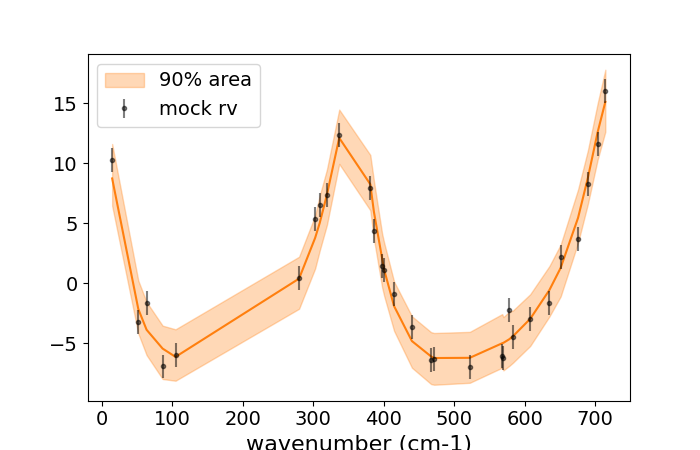
\includegraphics[width=\linewidth]{fig/rv_fit.png}
    \caption{Fit to the radial velocity data}
    \label{fig:rvfit}
\end{figure}
